\section{电阻率与温度和杂质浓度的关系}

尽管前面我们讨论的比较多的是电导率$\sigma$,但是因为半导体的电阻率可以通过四探针法直接读出,因此实践中更多的还是通过电阻率$\rho=\sigma^{-1}$来讨论问题,根据\xref{fml:半导体的迁移率与电导率}
\begin{Equation}
    \rho=\frac{1}{nq\mu_\text{n}+pq\mu_\text{p}}
\end{Equation}
电阻率同时取决于载流子的浓度和载流子的迁移率,因此,随杂质浓度和温度而异。

\subsection{电阻率与杂质浓度的关系}
\xref{fig:硅的电阻率和掺杂浓度的关系}给出了硅在室温下,电阻率与杂质浓度的关系。
\begin{Figure}[硅的电阻率和掺杂浓度的关系]
    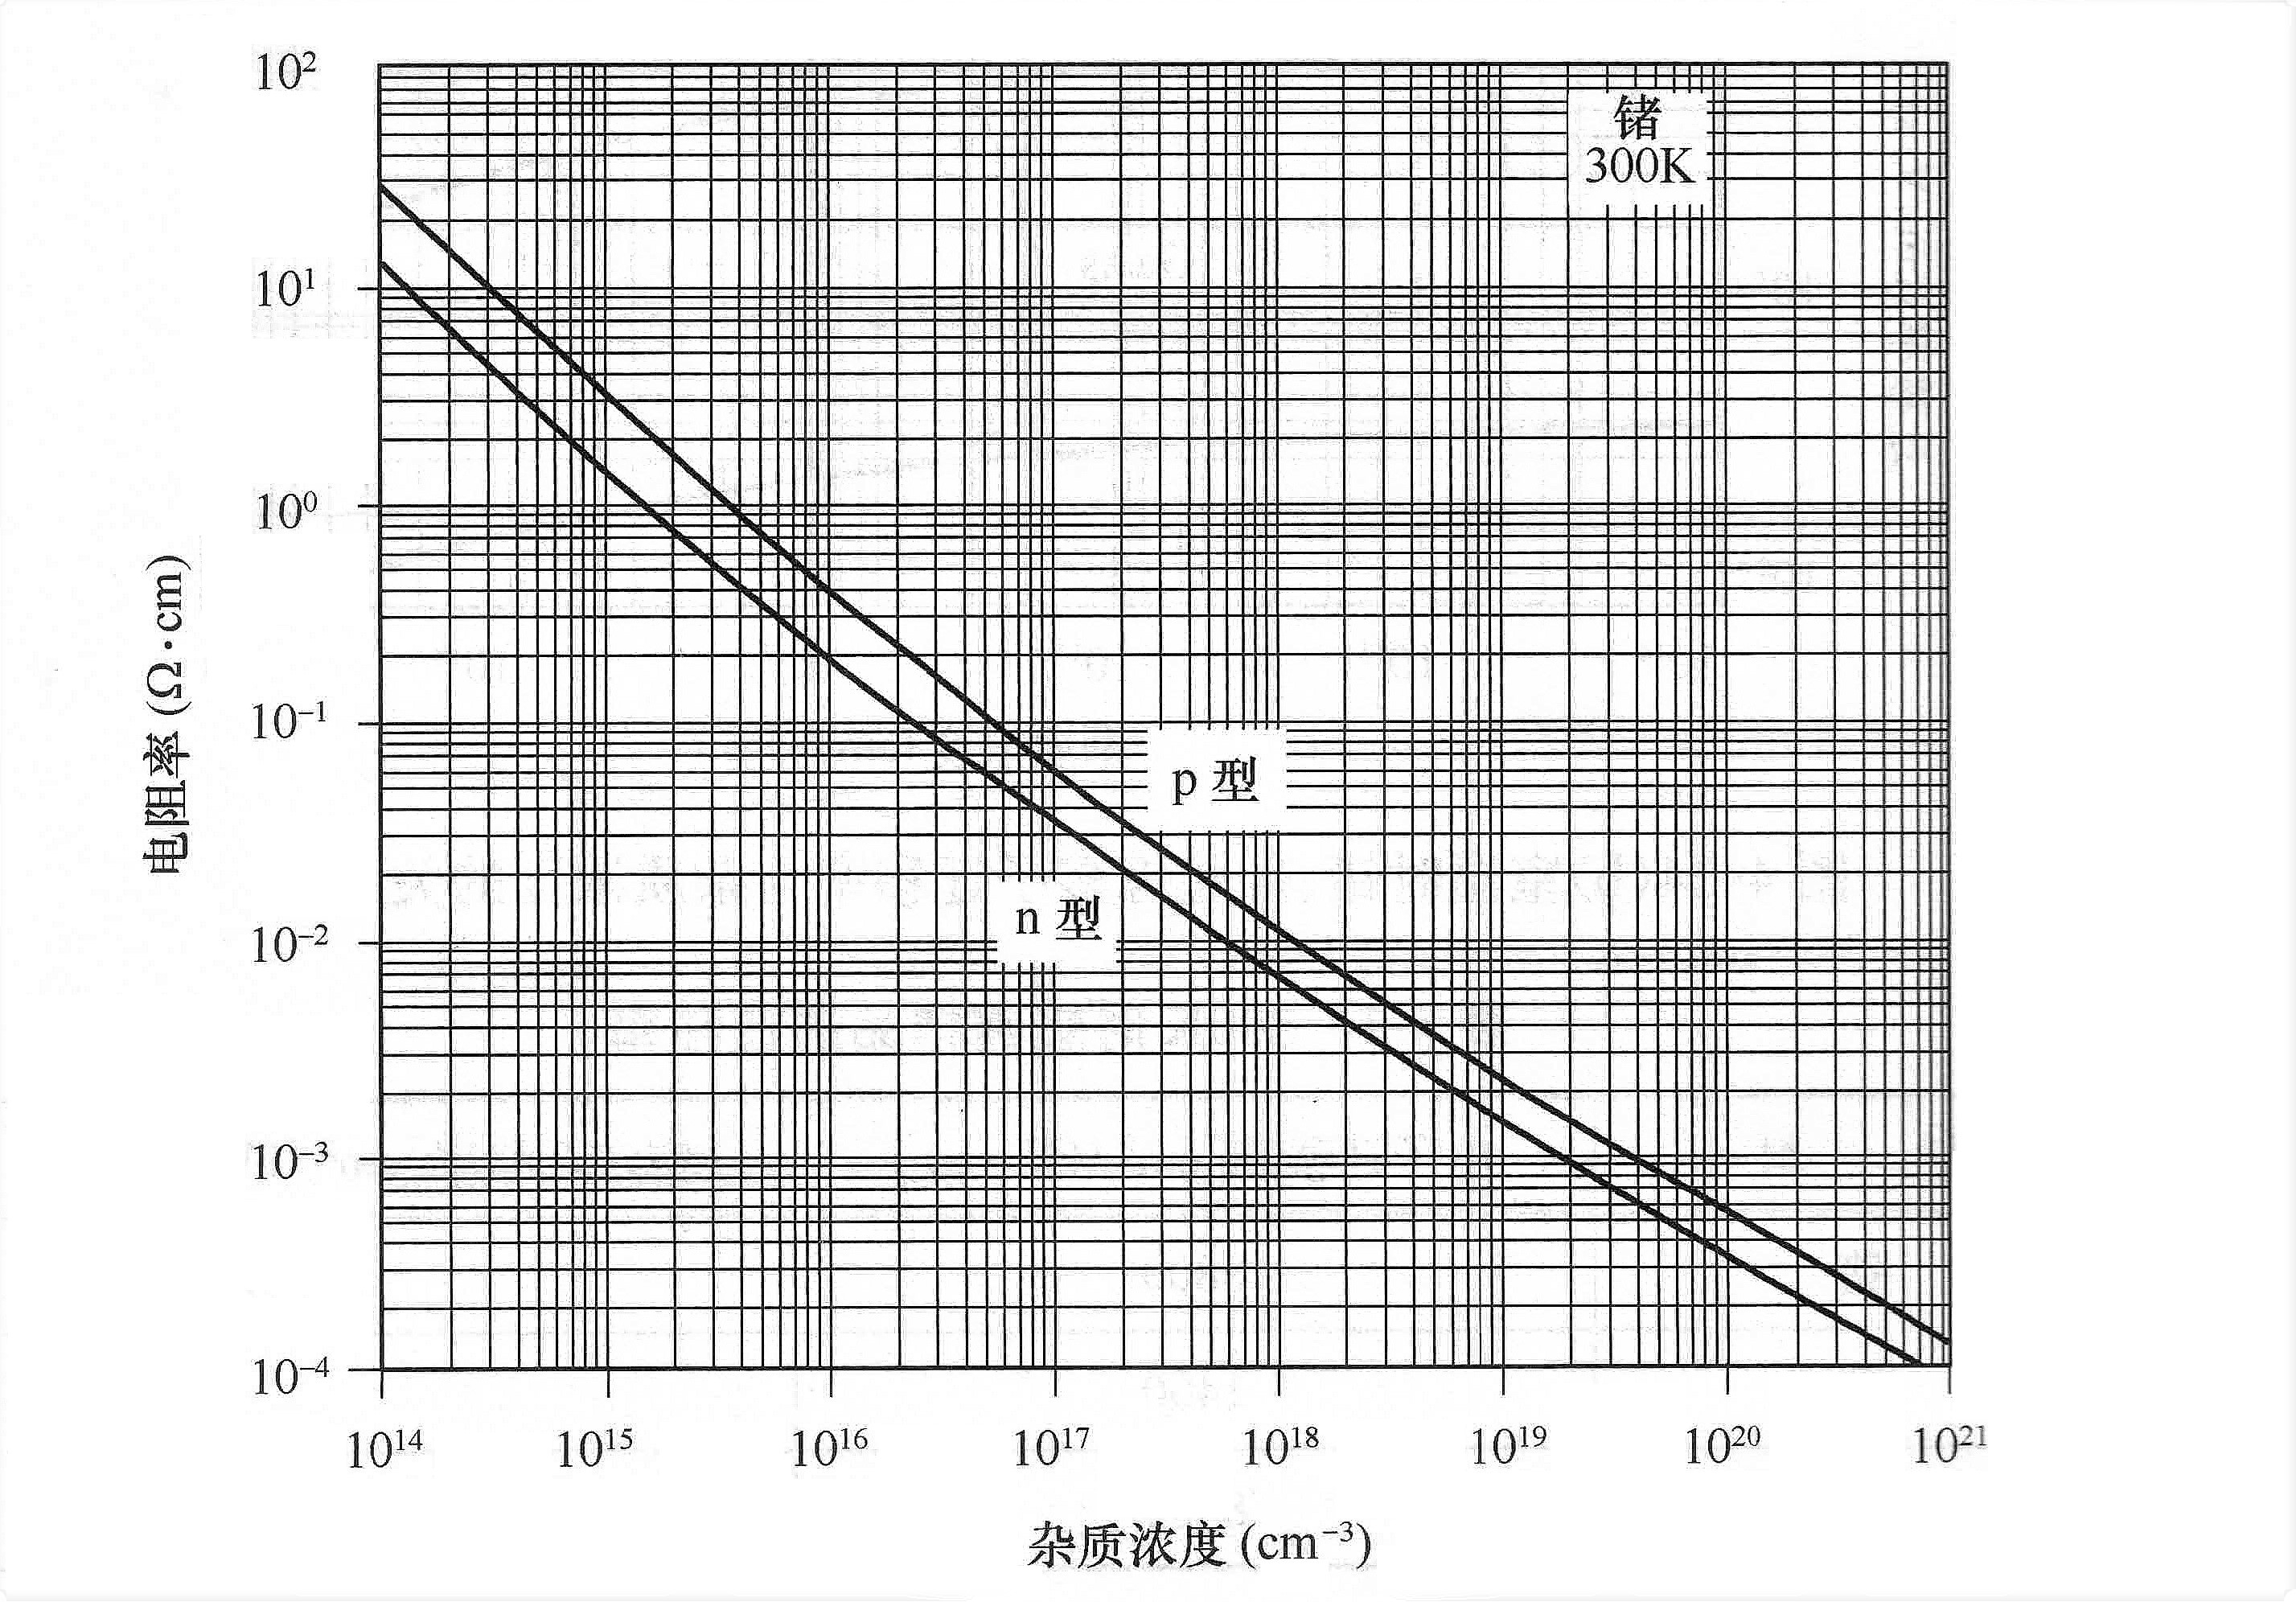
\includegraphics[width=12cm]{image/Ohm_Si.jpg}
\end{Figure}
轻掺杂时(杂质浓度低于$10^{18}\si{cm^{-3}}$),室温下杂质可以全部电离,即载流子浓度近似等于杂质浓度,即有$n=N_\text{D}$和$P=N_\text{A}$,同时如\xref{fig:硅的迁移率和掺杂浓度的关系},轻掺杂时迁移率可以近似为常数。因此,电阻率就与杂质浓度呈简单反比关系,反比关系在双对数坐标上,表现为斜率为$-1$的直线。

重掺杂时(杂质浓度高于$10^{18}\si{cm^{-3}}$),曲线则逐渐偏离原先的直线,这主要有两个原因
\begin{enumerate}
    \item 重掺杂时,杂质在室温下不能全部电离,并且会受到半导体简并的影响。
    \item 重掺杂时,迁移率将随杂质浓度的增加而显著下降。
\end{enumerate}
在室温下,本征硅的电阻率为$2.3\times 10^5\si{\ohm\cdot cm}$,本征锗的电阻率为$47\si{\ohm\cdot cm}$。


\subsection{电阻率与温度的关系}
对于本征半导体,电阻率主要由本征载流子浓度$n_\text{i}$决定,而$n_\text{i}$随温度增加急剧增加。

\begin{itemize}
    \item 对于本征硅,在室温附近,每增加$8\si{\degreeCelsius}\hphantom{1}$,硅的$n_\text{i}$增加一倍,电阻率降为一半。
    \item 对于本征锗,在室温附近,每增加$12\si{\degreeCelsius}$,硅的$n_\text{i}$增加一倍,电阻率降为一半。
\end{itemize}
因此,\empx{本征半导体的电阻率随温度增加而减小},这与金属导体是非常不同的。

对于杂质半导体,有杂质电离和本征激发两个因素存在,因而电阻率随温度的关系要复杂些
\begin{itemize}
    \item 在低温区,本征激发可以忽略,载流子主要由杂质电离提供,载流子浓度随温度升高而增加,同时,如\xref{fig:迁移率和温度的关系}所示,载流子的迁移率也随温度升高而增加,故电阻率下降。
    \item 在中温区(包括室温范围),本征激发仍然可以忽略,杂质则已全部电离,因此,载流子浓度不再变化,同时,散射方面,晶格振动散射取代电离杂质散射上升为主要矛盾,这样一来,如\xref{fig:迁移率和温度的关系}所示,载流子的迁移率将随温度升高而降低,故电阻率上升。
    \item 在高温区,本征激发占主导地位,回到本征半导体的情形,故电阻率下降。
\end{itemize}

总而言之,\empx{杂质半导体的电阻率随温度增加,先减小,再增加,再减小}。
